\documentclass[11pt,twocolumn]{article}
\usepackage[utf8]{inputenc}
\usepackage{graphicx} % Required for inserting images
\usepackage{multicol}
\usepackage{authblk}
\usepackage{hyperref}
\usepackage{titlesec}
\usepackage{amsmath}
\usepackage{amssymb}
\usepackage{natbib}
\bibliographystyle{abbrvnat}
\setcitestyle{authoryear,open={(},close={)},semicolon} %Citation-related commands
\makeatletter
\def\blfootnote{\xdef\@thefnmark{}\@footnotetext}
\makeatother

\titleformat{\section}[block]{\Large\bfseries\filcenter}{\thesection}{1em}{}

\title{\textbf {Domain Prompt Learning for Efficiently Adapting CLIP to Unseen Domains}}
\author[1]{\textbf{Xin Zhang}}
\author[1,2]{\textbf{Shiziang Shane Gu}}
\author[1]{\textbf{Yutuka Matsuo}}
\author[1]{\textbf{Yusuke Iwasawa}}
\affil[1]{The University of Tokyo}
\affil[2]{Google Research, Brain Team}

\begin{document}

\maketitle
\blfootnote{\url{xin@weblab.t.u-tokyo.ac.jp}}
\begin{abstract}
Domain generalization (DG) is a difficult transfer learning problem aiming to learn a generalizable model for unseen domains. Recent foundation models (FMs) are robust to many distribution shifts and, therefore, should substantially improve the performance of DG. In this work, we study generic ways to adopt CLIP, a Visual-Language Foundation Model, for DG problems in image classification. While ERM greatly improves the accuracy with bigger backbones and training datasets using standard DG benchmarks, fine-tuning FMs is not practical in many real-world situations. We propose DPL (Domain Prompt Learning) as a novel approach for domain inference in the form of conditional prompt generation. DPL achieved a significant accuracy improvement with only training a lightweight prompt generator (a three-layer MLP), whose parameter is of equivalent scale to the classification projector in the previous DG literature. Combining DPL with CLIP provides surprising performance, raising the accuracy of zero-shot CLIP from 73.7\% to 79.3\% on several standard datasets, namely PACS, VLCS, OfficeHome, and TerraIncognita. We hope the simplicity and success of our approach lead to broader adoption and analysis of foundation models in the domain generalization field. Our code is available at \url{https://github.com/shogi880/DPLCLIP}
\end{abstract}
\section{Introduction}
Pre-training large vision models using web-scale images is
an essential ingredient of recent success in computer vision. Fine-tuning pre-trained models, such as ResNet (He et al. 2015) and Vision Transformer (ViT) (Dosovitskiy et al. 2020) is the most popular paradigm for many downstream tasks. However, domain shifts pose a substantial challenge in real-world scenarios for successfully transferring models. Over the past decade, various studies on domain generalization (DG) have sought a systematic way to narrow the gap between source and target domains (Zhou et al. 2021a;Wang et al. 2021; Shen et al. 2021) aiming to build a model that generalizes to unseen domains. Despite the significant work on this front, machine learning systems are still vulnerable to domain shifts even after using DG methods (Gulrajani and Lopez-Paz 2020).
\newline
\begin{figure}
    \centering
    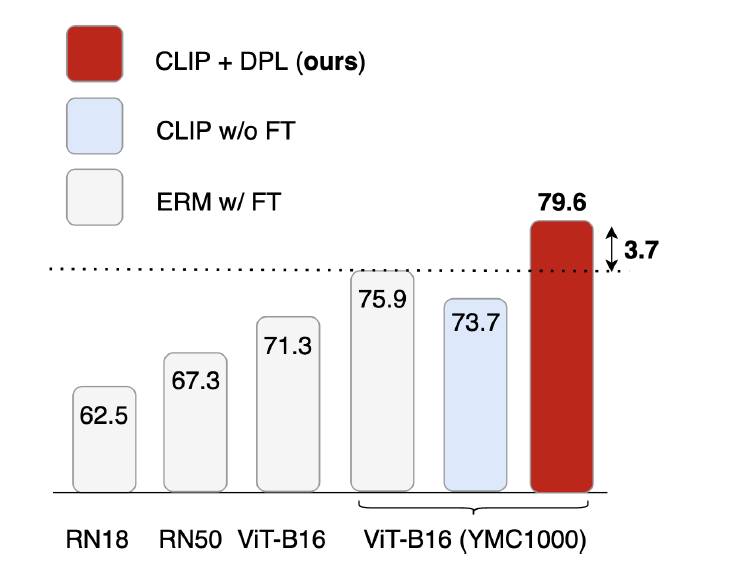
\includegraphics[width =0.5\textwidth]{Image1.png}
    \caption{Bigger backbone (from ResNet18 to ViT-B16) and bigger pre-train dataset (from ImageNet to YMC1000) improve the performance of ERM on VLCS, PACS, Office-Home, TerraIncognita. Even without fine-tuning the image encoder, our DPL (Domain Prompt Learning) effectively improves the performance of CLIP and outperforms the baseline ERM by a large margin (3.7\%). The CLIP w/o FT use the template prompt, such as ‘a photo of a {class name}’.}
    \label{fig:fig1}
\end{figure}
\hspace{1cm}
Large pre-trained vision-language models like Contrastive Language-Image Pre-Training (CLIP) are an emerging category of models showing great potential in learning transferable representation across many vision tasks. At the core of CLIP is to learn image representations by contrasting them with the representations of text description of the image, such as ‘a photo of a {class name}’. The text description is often called \textit{prompt}, and its design is vital in enhancing CLIP performance. Notably, CLIP can handle unseen classes without fine-tuning them by adequately changing the text description using the target class name. \\
\hspace{1cm}
This paper investigates the robustness of CLIP against various distribution shifts using DomainBed (Gulrajani and Lopez-Paz 2020), a recently proposed benchmark for DG setup. While prior works test various DG methods in the benchmark, the most studied only focused on medium-scale pre-trained models, such as ResNet18 or ResNet50. There are two na\"{\i}ve approaches to leveraging CLIP in the DG setup \autoref{fig:fig2} . The first approach is fine-tuning the image encoder trained by CLIP, similar to the other vision models such as ResNet and ViT. We show that the backbone networks trained by CLIP substantially outperform many backbone networks trained solely on images, such as ResNet, big transfer (Kolesnikov et al. 2020), and vision transformer (Dosovitskiy et al. 2020). At the same time, however, finetuning sometimes degraded the performance on some domains, suggesting that fine-tuning possibly distorts good properties of pre-trained features (Kumar et al. 2022). Another na\"{\i}ve approach is designing the template prompt, such as ‘a photo of a {class name}’. The clear merit of this approach is that it does not require optimizing any network and, therefore, keeps the representations learned via pretraining. Despite its simplicity, we show that zero-shot CLIP is still more robust on many DG benchmarks than the vision
backbones (e.g., ResNet18, ResNet50, ViT-B16) fine-tuned on source domains, while it is inferior to fine-tuning vision
backbone trained by CLIP.\\
\hspace{1cm}
Based on the observations, we propose Domain Prompt Learning (DPL), a simple yet effective extension of CLIP in the DG setup. A natural way to adapt the model is to add domain-specific features to the prompt template. However, manually designing a prompt template is challenging in many cases due to its ambiguity. Instead, we propose DPL for automatically generating a prompt that estimates domain-specific features given unlabeled examples from each distribution. More specifically, DPL trains a lightweight prompt generator using source domains, which outputs fixed-length continuous domain prompts given input images of each distribution while freezing other networks. During test-time, the prompt generator generates domain prompt given input images from the target distribution and adds them to the label prompts. Since the entire networks are frozen, the core properties of the pre-training would remain in DPL and are expected to improve CLIP performance in DG stably, as shown in our experiments.\\
\hspace{1cm}
It is worth noting our work is not the first attempt to tune the prompt of CLIP. For example, (Gao et al. 2021; Zhou et al. 2021b) have proposed optimizing continuous prompts on the target datasets, effectively improving CLIP performance. CoCoOp (Zhou et al. 2022), as a contemporary work, trains a meta-net to generate a meta token for adapting to each instance. CoCoOp focuses on unseen classes and demonstrates its performance by transferring from ImageNet to the four specially designed ImageNet variants. This work focuses on the robustness of CLIP against distribution shifts, and proposes a generic way to extract a domainspecific features and improve performance on the target domain at test-time.\\
\hspace{1cm}
We conduct experiments on four standard datasets included in DomainBed to evaluate DPL, following the experiment setup in(Gulrajani and Lopez-Paz 2020; Iwasawa and Matsuo 2021), such as parameter tuning and model selection. We show that CLIP with DPL outperforms the strong baselines by a large margin, raising the accuracy from 73.7\% to 79.6\% (Table 1). Moreover, since DPL can be seen as a kind of Test-Time Adaptation (TTA) method, we compare it with a series of SoTA TTA methods and demonstrate the efficiency of DPL (Table 2). And lastly, through various ablation studies, we surprisingly found that frozen backbone outperforms fine-tuning on OfficeHome datasets for all of ResNet, DeiT (Touvron et al. 2021), HViT, and ViT-B16 (Table 4). These results prove that DPL is effective, and more importantly, they provide many insights for future works that apply CLIP on DG.\\
\hspace{1cm}
In summary, our main contributions are:\\
\begin{enumerate}
    \item We introduce CLIP to standard DG benchmark DomainBed via prompt learning.\\
    \item We propose Domain Prompt Learning (DPL), a novel approach of domain inference, to effectively help domain
generalization by utilizing domain-specific features.\\
\item We demonstrate the impressive empirical performance of
DPL by comparing with strong DG baselines and a series
of state-of-the-art (SoTA) TTA methods.\\
\end{enumerate}
\begin{figure}
    \centering
    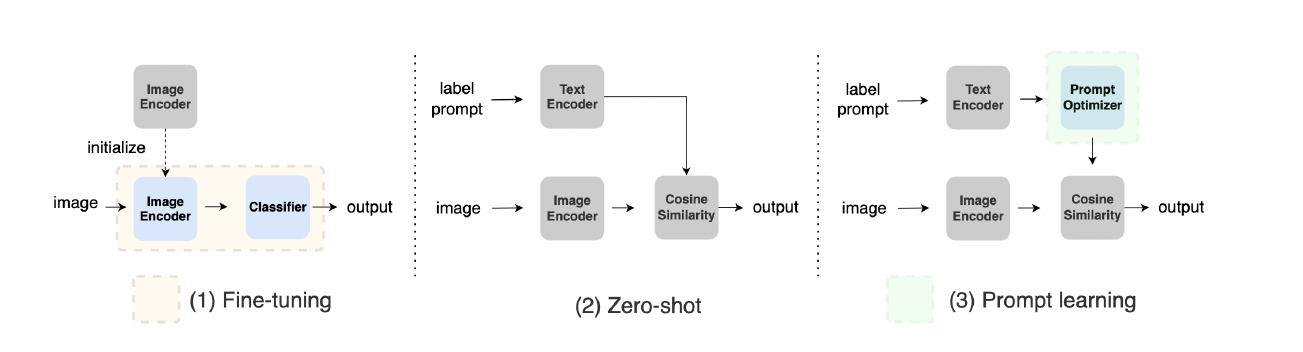
\includegraphics[width =0.5\textwidth]{Image2.png}
    \caption{The concept illustration of three approaches to apply CLIP in DG. (1) Fine-tuning updates the CLIP's image encoder with a trainable classifier. (2) Zero-shot CLIP contrastive prediction with hand-craft prompts at the test time without updating parameters on the train domains. (3) Prompt learning trains a prompt optimizer then utilize the optimized prompts to prediciton. Our DPL is categorized to (3) Prompt Learning, which trains a prompt generator in train phase and infers unseen domain to generate a domain-specific prompt.}
    \label{fig:fig2}
\end{figure}
\section{Method}
In this section, we first introduce the notations and definitions of DG following (Wang et al. 2021). Then, we explain how to use CLIP in DG and introduce Domain Prompt Learning to enhance CLIP performance in DG.
\subsection{Problem Setup of DG}
Let $\chi$ denote an input space and \begin{math}\mathcal{Y}\end{math} an output space. A domain is composed of data that has been sampled from a distribution. We denote the datasets from distribution as \begin{math}
S^i=(\mathbf{x}^i_j,y^i_j)_{j=1}^{n_i}\thicksim \mathcal{P}_{XY}^i
\end{math}, where \begin{math}
\mathbf{x} \in \chi \subset \Re^d \end{math} is an input image, 
\begin{math} \mathbf{y} \in \mathcal{Y}
\end{math} denotes the class associated with \begin{math}
    \mathbf{x}
\end{math}, and \begin{math}
    \mathcal{P}_{XY}^i
\end{math} denotes the joint distribution of the sample and output label in the domain $i$, X, Y denote the corresponding random variables.\\
\begin{figure}
    \centering
    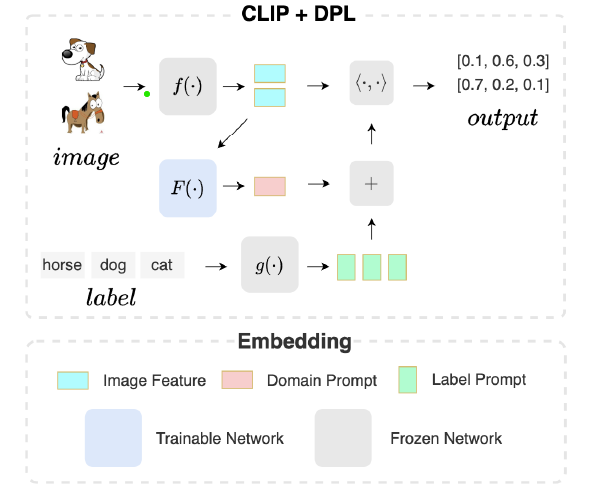
\includegraphics[width =0.5\textwidth]{Image3.png}
    \caption{The architecture of CLIP+DPL. The only one network we trained is the prompt generator $F(.)$, which is colored in blue. First, the input images are encoded to obtain image features with the frozen CLIP's image encoder $f(.)$. The image features are fed into the domain prompt generator $F(.)$ to generate a domain prompt. Simultaneously, all of labels are encoded using the frozen CLIP’s text encoder $g(.)$ to obtain the label prompt embeddings. Secondly, the domain prompt embeddings are added to the label prompt embeddings for calculating the similarity. Finally, to obtain the prediction output in probability, the cosine similarity $\langle .,. \rangle$ are calculated with image embeddings and domain prompt embeddings.}
    \label{fig:fig3}
\end{figure}
\hspace{1cm}
In DG, we are interested in predictor $h$ performance on data from an unseen domain \begin{math}\mathcal{P}_{XY}^i \neq \mathcal{P}_{XY}^i\end{math} for all $i$. Prior works fine-tuned a  pre-trained image encoder $f$ (usually ResNet18 or ResNet50) in conjunction with a randomly initialized classification head $g$ (linear classifier), using data from multiple different datasets to achieve the goal. Specifically, given $M$ datasets $S^i$ collected from various domains \begin{math}i \in {1,...,M}, f\end{math} and $g$ are updated by

\begin{equation}
    \min_{f,g} \frac{1}{M} \sum_{i=1}^{M} \frac{1}{n_i} \sum_{j=1}^{n_i} l(g \circ f(x_j^i),y_j^i),
\end{equation}

where $l$(.) is a loss function. In the simplest case, $l$ is a simple cross-entropy loss, and minimizing eq. \ref{eq:equation2} is called empirical risk minimization (ERM). As discussed in Section ??, different methods in DG use other loss functions by designing regularization terms to prevent overfitting specific domains. These datasets are frequently referred to as source domains, and they are distinguished as target domains where we want the model to perform well.

\subsection{Na\"{\i}ve Approaches for Using CLIP in DG}
CLIP consists of two parts: an image encoder $f_{clip}$ and a language model $g_{clip}$. CLIP classifies the image features based on the similarity between embedding of a text prompt $p$, such as 'dog' or 'a photo of a class label', rather than initially using the classification head trained from scratch. Specifically, given an image $x$ and $K$ class prompt $p_k$, CLIP output a prediction using both $f_{clip}$ and $g_{clip}$.

\begin{equation}
\label{eq:equation2}
    \hat{y}_{clip}=\arg \max_k \langle f_{clip}(x),g_{clip}(p_k)\rangle
\end{equation}
where $K$ is the number of categories and \textlangle.,.\textrangle is cosine similarity.\\
\hspace{1cm} To demonstrate how powerful the representation of massively pre-trained models (CLIP) for DG setup, we tested following two na\"{\i}ve approaches to use CLIP in DG setups: fine-tuning and zero-shot. Firstly, we evaluated CLIP in a zero-shot manner; i.e., we freeze both the image encoder and the language model, and substitute the class labels used in each dataset for the text prompt $p$.\\
\hspace{1cm} Secondly, we can use the image encoder $f_{clip}$ as an alternative to the standard image backbones, such as ResNet and ViT. In this setup, we train $f_{clip}$ by using the datasets $S^i$ from multiple source domains $i$, similar to the standard DG setup.We can use any algorithms tailored for DG setup, such as DANN and CORAL during fine-tuning. While it is powerful as shown in experiments, it requires additional computational costs to re-train such large models entirely. Besides, good properties of massive pre-training might be distorted
during fine-tuning, as highlighted by the performance degradation compared to zero-shot approach.\\
\hspace{1cm}
In summary, zero-shot approach is computationally effective yet less expressive, and fine-tuning can leverage the knowledge of source datasets but it is computationally heavy and possibly distort good representations learned during pretraining. Based on the observation, we propose a novel approach to design the prompt $p$ to improve the performance in an unseen domain without fine-tuning the entire model.

\subsection{Domain Prompt Learning for CLIP in DG}
As discussed in Section 2.3, designing a prompt is a powerful approach to improve the performance of the transformer based models. It is powerful and should also be easier to train because the dimension of prompts is significantly smaller than the entire parameters of $f$ and $g$. For example, supposing we can access a supervised dataset from the target domain, we can optimize a prefix vector $p_{pre}$ by simple supervised loss:
\begin{equation}
    \min_{p_{pre}} \mathbb{E}_{x,y\sim S}l(\hat{y}_{clip*},y),
\end{equation}
where $\hat{y}_{clip*}$ is
\begin{equation}
    \hat{y}_{clip*} = \arg \max_k \langle f_{clip}(x),g_{clip}(p_k^*)\rangle
\end{equation}
where $\textbf{\textit{p}}_k^*$ is a concatenation of trainable parameters $p_{pre}$ and $p_k$. Particularly, $g_{clip}$ outputs the fixed length vector regardless of the input dimension (i.e., size of $p_k$). The size of $p_k$ is a hyperparameter.\\
\hspace{1cm}
Unfortunately, this labeled training data for the target domain is unavailable in DG. Instead, we proposed DPL to replace the optimization process of $p_{pre}$ in each domain by training novel prompt generators $F(.)$ that generate a prompt $p_{pre}$ given small unlabeled images from a distribution. Specifically, we use a fully connected network $F(.)$ to generate prompt $p$ from input images:\\
\\
where $N$ is the batch size for each domain and $x_j^i$ denotes the images from the i-th distribution. Given a batch of data from multiple source distributions, we use the following loss function to optimize F:\\
\\
and \\
\\
where $p_k^i$ is a concatenation of pre-defined $p_k$ and$p_{ap}^i$.  The architecture of CLIP+DPL is depicted in \autoref{fig:fig3}.

\section{Conclusions}
We introduce CLIP to DG on DomainBed. For this purpose, we proposed a novel approach called Domain Prompt Learning (DPL) for efficiently adapting CLIP to an unseen domain. By generating the domain prompt conditional on input images, CLIP + DPL brings substantial improvements over strong DG baselines and several effective TTA methods on DomainBed. Then, we conducted ablation experiments with various backbones and Frozen ERM.We verified that DPL can stabilize performance and present meaningful insights about existing datasets and fine-tuning strategy of backbones. We hope that our research will broaden and inspire the roles of prompt learning in domain transfer learning.

\subsection{Limitation}
\label{subsec:5.1}
\textbf{Interpretability of Domain Prompt}  To better perform, our DPL is directly represented in a continuous vector form, which lacks interpretability. However, improving interpretability is an important research direction in both FM applications and Domain Generalization. We consider producing discrete semantically informative prompts by some means is an exciting extension of DPL, even with some loss of precision.\\
\textbf{Label Shift}    From the technical perspective, DPL cannot capture the domain shift outside of the images because DPL uses domain features extracted from only images. As a result, DPL has no idea how to record such non-visual domain shift. Unfortunately, the label shift exists in the actualworld applications \cite{azizzadenesheli2019regularized}. An innovative question is whether adding appropriate information to the Domain Prompt can help solve the label shift problem, such as a detailed textual description of the target domain.\\
\textbf{Social impact perspective}  Many images and text descriptions of web data are used directly to train CLIP. Though CLIP benefits from low-cost data that do not require manual labeling, it inevitably includes a lot of bias and privacy in CLIP and other foundation models \cite{bommasani2021opportunities}. This requires us to spend more time paying attention to the opportunities and risks of Foundation Models.

\subsection{Future Work}
First and foremost, interpretability is critical in both Domain Transfer Learning and the Foundation Model. As discussed in \autoref{subsec:5.1}, DPL introduce the possibility of using a large language model in DG in the form of prompt. We will investigate this direction in our future work.\\
\hspace{1cm}
There are two simple and critical approaches to improving the performance of DG. One is to apply visual prompt tuning \cite{jia2022visual} on the pure visual backbones, which can be used to more previous methods. Another is focusing on a data-centric approach since we observe uneven data quality on the widely used datasets.\\
\hspace{1cm}
Finally, several recent studies systematically analyze the performance and shortcomings of large-scale pre-train models in the Out-of-Distribution generalization \cite{cha2022domain,wenzel2022assaying}. We hope that our results will inspire more research in this direction.

\bibliography{namebib}
\end{document}
